\section{Comprehensive Evaluation}
The goal of the eviction policy is to control the memory usage of key-value cache under a fixed budget while retaining the generation quality of LLMs as much as possible. 
In this section, we perform an empirical evaluation of the effectiveness of various eviction policies by taking the generated output with a full KV cache as the reference and comparing KV-restricted generations against it.
\subsection{Experiment Setup}
We describe the experimental setup used throughout our evaluation, including evaluation tasks, metrics, datasets, and compared eviction policies.
\subsubsection{Tasks and Metrics}
\label{sec:tasks}
To broadly cover real-world use cases, we evaluate using four different types of tasks: language modeling, abstractive text summarization, original context reconstruction, and instruction following.
\paragraph{Language Modeling} Language modeling task assesses the ability of LLMs to predict the next token given the preceding context. In the key-value-constrained scenario, a successful eviction policy should be able to detect and remove KV cache of unimportant tokens. Following prior works~\cite{llminfinite,xiao2023efficient,tova}, we adopt perplexity as the evaluation metric.
\paragraph{Abstractive Text Summarization} Abstractive summarization requires extracting the most salient information provided in the input and generating a concise summary for it. Since the summary is usually much shorter compared to the input, we only perform cache eviction during the prefilling stage. We report BLEU~\cite{bleu}, ROUGE~\cite{rouge}, and METEOR~\cite{meteor} scores as the evaluation metrics.
\paragraph{Original Context Reconstruction} Given the constrained incomplete key-value cache of an input document, the task of original context reconstruction measures how well the limited KV cache retains the essential information from the original context. BLEU and ROUGE scores are used as evaluation metrics.
\paragraph{Instruction Following} Instruction following~\cite{flan} requires an LLM to generate a proper response for a given user instruction. We apply KV cache eviction at the auto-regressive decoding stage since the model output tends to be more verbose. In addition to BLEU and ROUGE scores, we also opt for a pairwise comparison paradigm to evaluate the generated responses against those generated by text-davincci-003.
\subsubsection{Datasets} 
We use the following datasets as the testbed for tasks described in \secref{sec:tasks}.
\paragraph{OpenWebText} OpenWebText is an open-source replication of the WebText dataset from OpenAI. We randomly sample 200 documents to form the test set for the language modeling task.
\paragraph{XSum} Xsum~\cite{xsum} comprises BBC articles from the years 2010 to 2017, encompassing a broad spectrum of topics.
\paragraph{CNN/Daily Mail} CNN/Daily Mail~\cite{cnndm} contains articles from the CNN and the Daily Mail newspapers, representing a different distribution from XSum. We use this dataset for both summarization and original context reconstruction.
\paragraph{AlpacaEval} AlpacaEval~\cite{alpaca_eval} is a model-based automatic evaluation benchmark for instruction-following LLMs. It comprises 805 instructions spanning a diverse range of scenarios.
\subsubsection{Models}
Following prior works~\cite{h2o,tova}, we employ LLaMa2-7B-base for language modeling and LLaMa2-7B-Chat for the remaining tasks. We also include WizardLM-7B~\cite{wizardlm} as another strong instruction-tuned LLM for tasks except for language modeling.

\subsubsection{Compared Eviction Policies}
\begin{table}[h]
    \small
    \centering
    \begin{tabular}{l|cc}
     \toprule
     & \multicolumn{1}{l}{\textbf{Importance Score}} & \multicolumn{1}{l}{\textbf{Eviction Scope}} \\
     \midrule
    Random       & -    & -                \\
    StreamLLM   & -    & local window    \\
    ScissorHands & AQAS & local window       \\
    H$_{\text{2}}$O          & AAS  & local window       \\
    TOVA         & LTAS & -                \\
    RoCo         & MAS  & standard deviation \\
    \bottomrule
    \end{tabular}
    \caption{Eviction policies considered in this paper. The definition of importance score and eviction scope are introduced in \secref{sec:isc} and \secref{sec:esc}, respectively.}
    \label{tab:policies}
\end{table}
\begin{table*}[t]
    \centering
    \small
    \begin{tabular}{cc|ccccc|ccccc}
    \toprule
    \multicolumn{1}{c}{\multirow{2}{*}{\textbf{Models}}} & \multirow{2}{*}{\textbf{Methods}} & \multicolumn{5}{c}{\textbf{XSum}}         & \multicolumn{5}{c}{\textbf{CNN/DM}}       \\
    \multicolumn{1}{c}{} &              & BLEU & Meteor & R-1  & R-2  & R-L  & BLEU & Meteor & R-1  & R-2  & R-L  \\
    \midrule
    \multirow{6}{*}{LLaMa2-7B$_{\text{chat}}$}             & Random                   & 16.7 & 35.1 & 41.8 & 22.8 & 33.3 & 15.4 & 30.8 & 39.0 & 19.9 & 26.2 \\
                         & StreamLLM   & 11.9 & 35.5   & 42.7 & 17.6 & 31.3 & 19.2 & 40.0   & 49.5 & 24.3 & 30.7 \\
                         & ScissorHands & 29.3 & 50.4   & 56.5 & 35.6 & 46.5 & 27.8 & 46.4   & 57.7 & 33.4 & 40.7 \\
                         & H$_{\text{2}}$O          & 37.3 & 55.8   & 62.2 & 44.2 & 54.2 & 31.1 & 47.6   & 58.9 & 36.8 & 43.7 \\
                         & TOVA         & 20.5 & 42.4   & 48.9 & 26.9 & 39.9 & 21.5 & 41.7   & 53.1 & 27.4 & 34.8 \\
                         & RoCo         & \textbf{43.4} & \textbf{60.5}   & \textbf{65.0} & \textbf{48.6} & \textbf{57.8} & \textbf{33.2} & \textbf{49.3}   & \textbf{61.1} & \textbf{39.2} & \textbf{46.0} \\
    \midrule
    \multirow{6}{*}{WizardLM-7B}             & Random                   &12.6  &30.0  &36.3  &19.1  &28.0  &12.4  &27.8  &39.6  &17.0  &23.9  \\
                         & StreamLLM   &7.1  &27.3    &36.2  &13.4  &25.6  &8.8  &25.9    &39.0  &14.4  &23.8  \\
                         & ScissorHands &29.8  &48.6    &57.2  &38.5  &47.7  &24.6  &41.2    &54.3  &29.1  &35.7  \\
                         & H$_{\text{2}}$O          &30.5  &50.2    &57.6  &40.8  &49.7  &27.7  &43.3    &56.4  &32.5  &39.2  \\
                         & TOVA         &15.0  &36.2    &46.1  &23.9  &34.8  &14.5  &32.7    &45.9  &19.4  &27.9  \\
                         & RoCo         &\textbf{35.7}  &\textbf{56.6}    &\textbf{61.4}  &\textbf{45.5}  &\textbf{53.7}  &\textbf{30.2}  &\textbf{45.9}    &\textbf{59.1}  &\textbf{35.6}  &\textbf{42.4}  \\
    \bottomrule
    \end{tabular}
    \caption{Performance of different eviction policies on abstractive text summarization tasks at 0.5 KV cache rate.}
    \label{table:sum}
\end{table*}
We consider the following baseline eviction policies, with their importance score calculation methods and eviction scope listed in \tabref{tab:policies}:
\begin{itemize}[itemsep=1pt,parsep=2pt,topsep=1pt]
    \item Random: evicting a randomly selected key-value pair from the cache.
    \item StreamLLM~\cite{xiao2023efficient}: evicting the key-value pair corresponding to the first token after 4 initial attention sink tokens.
    \item ScissorHands~\cite{liu2023scissorhands}: evicting the key-value pair corresponding to the token with the smallest accumulative quantized attention score outside the local window of size $r$.
    \item H$_{\text{2}}$O~\cite{h2o}: evicting the key-value pair corresponding to the token with the smallest accumulative attention score outside of the local window of size $r$.
    \item TOVA~\cite{tova}: evicting the key-value pair corresponding to the token with the smallest last token attention score.
\end{itemize}
\subsubsection{Other Details}
Our implementation is based on Pytorch~\cite{pytorch} and HuggingFace Transformers~\cite{wolf-etal-2020-transformers}. To improve the stability of outputs produced by LLMs, we employ greedy decoding for all generative tasks. For prefilling stage eviction, we set budget size $B$ by multiplying input token length with a compression rate~(e.g., 0.5) and directly specify $B$ as some integer for decoding stage eviction because the output length is unknown. The size of the local window is set to half of the KV cache budget following H$_{\text{2}}$O, i.e. $r=B/2$.
\begin{figure}[t]
	\centering
	\scalebox{0.41}{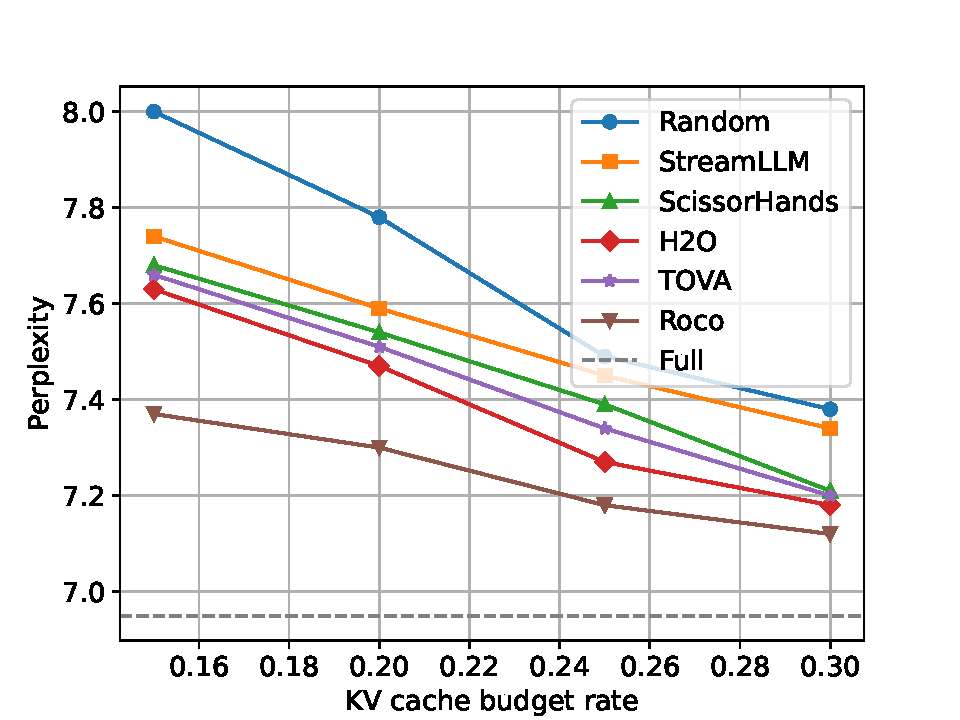
\includegraphics{./figures/ppl.pdf}}
    \caption{Performance of different eviction policies on language modeling task based on LLaMa2-7B.}
	\label{fig:ppl}
\end{figure}
\begin{table}[t]
    \centering
    \small
    \begin{tabular}{cc|ccc}
    \toprule
    \multirow{2}{*}{\textbf{Models}}    & \multirow{2}{*}{\textbf{Methods}} & \multicolumn{3}{c}{\textbf{CNN/DM}} \\
                               &                          & BLEU   & R-1  & R-L  \\
    \midrule
    \multirow{6}{*}{LLaMa2-7B$_{\text{chat}}$} & Random                   &4.9             &26.7      &18.1      \\
                               & StreamLLM                &15.1             &37.6      &28.5      \\
                               & ScissorHands             &16.9             &45.9      &33.7      \\
                               & H$_{\text{2}}$O                      &20.8             &50.6      &40.7      \\
                               & TOVA                     &11.2             & 43.1     &30.3      \\
                               & RoCo                     & \textbf{28.1}            &\textbf{57.7}      &\textbf{49.2}      \\
    \midrule
    \multirow{6}{*}{WizardLM-7B} & Random                   &6.3             &30.3      &19.6      \\
                               & StreamLLM                &5.3             &24.7      &16.3      \\
                               & ScissorHands             &17.4             &48.3      &33.0      \\
                               & H$_{\text{2}}$O                      &20.8             &50.8      &38.5      \\
                               & TOVA                     &12.5             &41.7      &27.7      \\
                               & RoCo                     &\textbf{29.0}             &\textbf{58.9}      &\textbf{47.5}      \\
    \bottomrule
    \end{tabular}
    \caption{Performance of different eviction policies on context reconstruction task at 0.5 KV cache rate.}
    \label{table:rec}
\end{table}
\begin{table*}[t]
    \centering
    \small
    \begin{tabular}{cc|cccc}
    \toprule
    \multicolumn{1}{c}{\multirow{2}{*}{\textbf{Models}}} & \multirow{2}{*}{\textbf{Methods}} & \multicolumn{4}{c}{\textbf{AlpacaEval}}               \\
    \multicolumn{1}{c}{} &              & BLEU & ROUGE-1  & ROUGE-2  & ROUGE-L  \\
    \midrule
    \multirow{6}{*}{LLaMa2-7B$_{\text{chat}}$}             & Random                   &45.6  &66.6  &49.7  &56.1     \\
                         & StreamLLM   &47.3  &66.6    &51.1  &57.1    \\
                         & ScissorHands &62.1  &76.5    &63.9  &68.8     \\
                         & H$_{\text{2}}$O          &63.0  &77.5   &65.7  &69.9      \\
                         & TOVA         &60.1 &75.3    &63.8  &68.3    \\
                         & RoCo         &\textbf{66.3}  &\textbf{79.7}    &\textbf{68.1}  &\textbf{72.5}     \\
    \midrule
    \multirow{6}{*}{WizardLM-7B}             & Random                   &40.6  &62.9  &45.6  &52.8     \\
                         & StreamLLM   &43.0  &63.9    &47.8  &54.5     \\
                         & ScissorHands &57.2  &73.3    &60.9  &65.3     \\
                         & H$_{\text{2}}$O          &58.6  &74.1    &62.1  &66.8     \\
                         & TOVA         &59.6  &75.0    &63.1  &68.0     \\
                         & RoCo         &\textbf{62.2}  &\textbf{76.4}    &\textbf{64.5}  &\textbf{69.5}    \\
    \bottomrule
    \end{tabular}
    \caption{Performance of different eviction policies on AlpacaEval at 250-token KV cache budget.}
    \label{table:alpacaeval}
\end{table*}
\subsection{Main Results}
\begin{table}[t]
    \centering
    \small
    \begin{tabular}{cccc}
    \toprule
    \textbf{Budget} & \textbf{StreamLLM} & \textbf{H$_{\text{2}}$O} & \textbf{RoCo} \\
    \midrule
    200              & 72.0(-3.6)               & 74.5(-1.1)         & 75.2(-0.4)          \\
    250              & 72.9(-2.7)               & 74.8(-0.8)         & 75.5(-0.1)          \\
    \bottomrule
    \end{tabular}
    \caption{AlpacaEval win rates against text-davincci-003 judged by GPT-4. Numbers in the parenthesis denote the performance drop compared to full KV cache~(500 token output length on average with 75.6 win rate).}
    \label{table:gpt4}
\end{table}
\paragraph{Overview} We report the results of RoCo alongside compared baseline eviction policies on language modeling, text summarization, original context reconstruction, and instruction following tasks in \figref{fig:ppl}, \tabref{table:sum}, \tabref{table:alpacaeval}, and \tabref{table:rec}. 
It can be seen that RoCo consistently outperforms previous methods by significant margins across all tasks and models. The advantage of Roco is particularly more evident at a low KV cache budget rate. As demonstrated in \figref{fig:ppl}, the gap between Roco and the second best method H$_{\text{2}}$O reaches 0.2 at 0.15 budget rate. We also notice that Roco yields larger improvements on generative inference tasks compared to language modeling. This is because, in generative tasks, future token predictions are dependent on previous model generations, where minor errors can accumulate and lead to large divergence. 
on the AlpacaEval benchmark, RoCo not only delivers the best overall performance in conventional metrics like BLEU and ROUGE, but also achieves comparable win rates as judged by GPT-4~(\tabref{table:gpt4}). In contrast, H$_{\text{2}}$O shows notable quality declines, and the gap is even larger for StreamLLM. Overall, the experiment results validate the effectiveness of Roco in terms of retaining model performance during key-value-constrained inference.
\paragraph{Attention Matters for KV Eviction} As the only two policies that do not utilize attention-related information, Random and StreamLLM show significantly inferior performance compared to attention-based methods on all tasks. This observation aligns with the role of key-value vectors in attention computation, where the attention score serves natural indicator of token importance.
\subsection{Discussion}
\paragraph{Extension to Grouped-Query Attention~(GQA)} GQA, along with its extreme case Multi-Query Attention~(MQA) has gained increasing adoption in powerful LLMs like Mistral~\cite{mistral}. We extend the attention-based eviction policy to GQA and MQA by taking the group-wise averaged attention score and using it to update the importance score according to \secref{sec:isc}. The results of Zephyr-7B~\cite{tunstall2023zephyr} in Appendix \ref{sec:appendix_a} validate the effectiveness of our extension.
\paragraph{Overhead} An ideal eviction policy should avoid introducing much extra overhead since LLMs are already memory and computational-intensive. The memory overhead induced by Roco is $L\times H\times B\times 3$, which is negligible given the reduced KV cache footprint $L\times 2\times H\times (S-B)\times d^\prime$, where $S$ is the non-evicted full sequence length. Moreover, different from the auto-regressive decoding stage which is I/O-bounded, the prefilling stage is computation-bounded. However, prior policies usually evict one token every time the cache is full and encode the next token, turning the prefilling stage into I/O-bounded. To accelerate key-value constrained prompt encoding, RoCo allows for performing evict-and-encode in a block-wise manner. The block size $b$ controls the number of tokens being freed and encoded within one eviction step. We examine the effect of block-wise eviction using LLaMa2-7B-Chat on XSum summarization task. \tabref{table:blockwise} shows that such block-wise eviction greatly speeds up prefilling while retaining similar output quality as token-wise eviction. More results are deferred to Appendix \ref{sec:appendix_b} due to space limit.
\begin{table}[t]
    \centering
    \small
    \begin{tabular}{cccc}
    \toprule
    \textbf{Block Size} & \textbf{BLEU} & \textbf{ROUGE-2} & \textbf{Speed up} \\
    \midrule
    1                   & 41.2          & 46.2             & 1.0x              \\
    2                   & 41.1          & 46.3             & 2.0x              \\
    4                   & 41.1          & 46.2             & 4.0x              \\
    8                   & 40.4          & 45.5             & 8.0x              \\
    16                  & 40.2          & 45.4             & 16.0x             \\
    \bottomrule
    \end{tabular}
    \caption{Summarization results of block-wise eviction using RoCo. }
    \label{table:blockwise}
\end{table}
\paragraph{Integrated Package} Finally, we open-source EasyKV, a software package dedicated to key-value constrained inference accompanying this research. It is designed to be fully compatible with existing LLMs with different attention variants and enables flexible configuration of diverse eviction policies, cache budgets, and application scenarios.
